\documentclass[conference]{IEEEtran}
\IEEEoverridecommandlockouts

\usepackage{cite}
\usepackage{amsmath,amssymb,amsfonts}
\usepackage{algorithm}
\usepackage{algpseudocode}
\usepackage{graphicx}
\usepackage{textcomp}
\usepackage{xcolor}
\usepackage{listings}
\usepackage{booktabs}
\usepackage{multirow}
\usepackage{url}
\usepackage{array}
\usepackage{float}
\usepackage{tabularx}
\usepackage{caption}
\usepackage[utf8]{inputenc}



% Define the 'P' column type for centered paragraphs with fixed width
\newcolumntype{P}[1]{>{\centering\arraybackslash}p{#1}}

% Setup for code listings
\lstset{
    language=C,
    basicstyle=\ttfamily\footnotesize,
    breaklines=true,
    frame=single,
    captionpos=b,
    keywordstyle=\color{blue},
    commentstyle=\color{gray},
    stringstyle=\color{red},
    numbers=none,
    columns=fullflexible,
    keepspaces=true,
    xleftmargin=2pt,
    xrightmargin=2pt,
    aboveskip=4pt,
    belowskip=2pt
}

\begin{document}

% --- TITLE ---
\title{Empirical Analysis of Optimization Phase Ordering
Trade-offs in a Custom Compiler Using
Micro-Benchmarks}

\author{
    \makebox[\textwidth][c]{%
        \begin{minipage}[t]{0.3\textwidth}
            \centering
            \text{Aniket De}\\
            \textit{Dept. of Computer Science and Engineering}\\
            \textit{Sahyadri College of Engineering \& Management}\\
            Mangaluru, India\\
            aniketde66@gmail.com
        \end{minipage}
        \hfill
        \begin{minipage}[t]{0.3\textwidth}
            \centering
            \text{Kushal S M}\\
            \textit{Dept. of Computer Science and Engineering}\\
            \textit{Sahyadri College of Engineering \& Management}\\
            Mangaluru, India\\
            mrkushalsm@gmail.com
        \end{minipage}
        \hfill
        \begin{minipage}[t]{0.3\textwidth}
            \centering
            \text{Manas S}\\
            \textit{Dept. of Computer Science and Engineering}\\
            \textit{Sahyadri College of Engineering \& Management}\\
            Mangaluru, India\\
            salianmanas@gmail.com
        \end{minipage}
    }\\[2ex]

    \makebox[\textwidth][c]{%
        \begin{minipage}[t]{0.4\textwidth}
            \centering
            \text{Vivek Neeralagi}\\
            \textit{Dept. of Computer Science and Engineering}\\
            \textit{Sahyadri College of Engineering \& Management}\\
            Mangaluru, India\\
            vivekneeralagi@gmail.com
        \end{minipage}
        \hfill
        \begin{minipage}[t]{0.4\textwidth}
            \centering
            \text{Dr. Suhas A Bhyratae}\\
            \textit{Dept. of Computer Science and Engineering}\\
            \textit{Sahyadri College of Engineering and Management}\\
            Mangaluru, India\\
            suhasabhyraatae.cs@sahyadri.edu.in
        \end{minipage}
    }
}

\maketitle

% --- ABSTRACT ---
\begin{abstract}
The phase ordering problem, the dependence of optimization results on the order in which compiler passes are applied, is a long-standing issue in compiler design. This paper reports a controlled, exhaustive study of the problem on a purpose-built compiler. The compiler has a handwritten lexical analyzer, a recursive-descent parser, and a Three-Address Code (3AC) intermediate representation, and it implements six classical passes (Constant Folding, Dead Code Elimination, Common Subexpression Elimination, Copy Propagation, Strength Reduction, and Algebraic Simplification) as independent, reorderable units under a configurable pass manager. All 720 orderings of the six passes were applied to fifteen micro-benchmarks adapted from MiBench and PolyBench/C, giving 10,815 optimized programs, each verified to print the same output as its unoptimized baseline. Three metrics were recorded: static instruction count, an estimated cycle cost under a stated per-instruction cost model, and the dynamic instruction count from an IR interpreter. The best family of orderings reduces code size by a geometric mean of 35.7\% (22\% to 60\% per program), estimated cycles by 20.5\%, and executed instructions by 23.2\%, whereas a third of all orderings reduce code size by only 1.3\%. The 720 orderings collapse into nine equivalence classes fixed by the relative order of four passes, and the same relative order is optimal on every program. The effect of ordering is significant across programs (Friedman test, $p < 10^{-48}$, Kendall's $W = 0.88$). The cost model, the derivation of the pass-interaction matrix, and the baseline program are given in full so that the results can be reproduced from the released source.
\end{abstract}

% --- KEYWORDS ---
\begin{IEEEkeywords}
Common Subexpression Elimination,
Compiler Optimization,
Constant Folding,
Dead Code Elimination,
Micro-Benchmarking,
Phase Ordering Problem,
Three-Address Code
\end{IEEEkeywords}

\section{Introduction}

Compilers are fundamental components of modern computing systems that translate high-level programming languages into machine-executable code \cite{ref21}. The quality of generated code directly affects execution speed, memory usage, and overall system efficiency \cite{ref18}. As software systems become more complex and are deployed in resource-constrained environments, efficient compiler optimization becomes essential.

Compiler optimization techniques aim to improve program performance without changing its functionality \cite{ref21}. Common methods such as Constant Folding, Dead Code Elimination, and Common Subexpression Elimination reduce redundant computations and unnecessary instructions \cite{ref18}. However, the effectiveness of these optimizations depends on the order in which they are applied during compilation \cite{ref19}.

This leads to the \textit{Phase Ordering Problem}, a major challenge in compiler design \cite{ref1}. It refers to determining the sequence of optimization passes that gives the best performance and the smallest code \cite{ref2}. Different orderings of the same optimizations can produce different results, because some passes expose opportunities for others while some destroy them \cite{ref19}. The number of possible orderings grows factorially with the number of passes, so exhaustive evaluation is impractical in production compilers \cite{ref2}.

Modern compilers such as LLVM and GCC address this problem using predefined optimization pipelines guided by heuristics \cite{ref16}. While effective in practice, these pipelines are large and tightly coupled, which makes it difficult to isolate the effect of a single ordering decision \cite{ref16}.

This paper takes the opposite approach. It uses a small compiler in which six classical passes are implemented so that each one is valid in any position, and it measures every one of the $6! = 720$ orderings on fifteen micro-benchmarks. The compiler includes a handwritten lexical analyzer, a recursive-descent parser, and a Three-Address Code (3AC) intermediate representation on which the passes operate \cite{ref18}. Each configuration is measured by static instruction count (code size), an estimated cycle cost (a static model of runtime), and the number of instructions actually executed by an IR interpreter.

The six passes are textbook transformations \cite{ref18,ref21}; the contribution of this paper is the measurement, not the passes. Specifically, the paper contributes: (1) an infrastructure in which every pass is block-local and side-effect free, so that all 720 orderings can be run and compared without a correctness caveat; (2) an exhaustive, output-validated evaluation of all orderings on fifteen MiBench- and PolyBench-derived kernels under three metrics; (3) the empirical structure of the ordering space, namely nine equivalence classes, four ordering rules, and a quantified cost of a poor order; and (4) a full specification of the metrics, the cost model, and the interaction-matrix derivation, with the source code released\footnote{\url{https://github.com/VivekNeer/major-project-compiler-design}}, so that every table in the paper can be regenerated with one command.

% --- SECTION II: LITERATURE REVIEW ---

\section{Literature Survey}

The phase-ordering problem is a long-standing open issue in compiler optimization research \cite{ref1}. The ordering of compiler optimization passes influences both execution performance and generated code size \cite{ref2}. However, the exponential growth of possible optimization sequences makes exhaustive exploration impractical for real-world systems \cite{ref19}.

\subsection{Dependency-Based and Pruning Approaches}
Several techniques have been proposed to reduce the complexity of the phase-ordering search space. Dependency-based modeling approaches attempt to identify relationships between optimization passes to improve overall efficiency \cite{ref1}. Liu et al. demonstrated that explicitly modeling pass dependencies can improve optimization effectiveness by reducing redundant transformations \cite{ref1}. Similarly, pruning-based strategies eliminate low-impact transformations and retain only high-value optimization combinations, reducing unnecessary exploration overhead \cite{ref4}. While these methods improve performance, they often depend heavily on predefined heuristics and structural assumptions \cite{ref19}.

\subsection{Machine Learning Methods}
Machine learning\textendash based compiler autotuning is the other main line of work. Predictive models analyze application features and dynamically select optimization passes to improve execution performance \cite{ref8}. Reinforcement learning\textendash based frameworks such as POSET-RL demonstrate improved optimization selection by adapting optimization sequences based on runtime feedback \cite{ref8}. Similarly, AutoPhase introduced learning-driven phase ordering mechanisms that optimize transformation sequences in high-level synthesis environments \cite{ref12}. These methods improve search efficiency but add training overhead and depend on large datasets \cite{ref12}. Related work in this direction includes learned program embeddings for optimization decisions \cite{ref9}, predictive and ensemble models for selecting flags or phases \cite{ref17,ref22,ref28,ref29}, graph-based iterative pass selection \cite{ref20}, and techniques that enlarge or restructure the search space itself, such as dormant-information learning \cite{ref26}, booster pass chains \cite{ref25}, and search for globally optimal code across phases \cite{ref3}.

\subsection{Industrial Compiler Frameworks}
The LLVM compilation infrastructure introduced a modular and extensible intermediate representation that supports continuous program transformation and analysis \cite{ref16}. However, large-scale production compilers typically involve tightly coupled optimization pipelines, making it difficult to isolate and analyze individual pass interactions in controlled environments \cite{ref16}. Within such compilers, run-time data \cite{ref23} and comparison of optimization decisions across runs \cite{ref24} have been used to diagnose and steer optimizations.

Recent research has explored advanced optimization strategies that integrate statistical modeling and automated selection methods. Zhao et al. introduced statistical-based frameworks to predict profitable optimization sequences using compilation metadata \cite{ref7}. Similarly, recent work by Ashouri et al. proposed agile compiler frameworks capable of dynamically adapting optimization pipelines for improved performance \cite{ref27}. Although these approaches demonstrate improved efficiency, they remain computationally intensive and less suitable for simplified educational or experimental compiler systems \cite{ref27}.

\subsection{Identifying the Research Gap}
Most of the work above optimizes for performance and treats the pass pipeline as a black box \cite{ref2}. Kulkarni et al. observed that many phase sequences produce identical code and that, for a small pass set, the distinct outcomes can be enumerated exhaustively \cite{ref19}; the present study relies on exactly this property. Visualization tools for teaching compiler optimizations \cite{ref30} address transparency but do not measure ordering effects. There remains a need for simplified compiler infrastructures that enable controlled experimentation and empirical analysis of optimization ordering behavior \cite{ref1}. Such frameworks make it possible to measure, rather than estimate, the trade-off between execution performance and code size for a given set of passes \cite{ref19}.

\begin{table}[htbp]
\caption{Comparative Analysis of Related Work}
\label{tab:lit_review}
\centering
\renewcommand{\arraystretch}{1.1}
\begin{tabularx}{\columnwidth}{@{}p{0.22\columnwidth} p{0.22\columnwidth} X@{}}
\toprule
\textbf{Reference} & \textbf{Focus Area} & \textbf{Limitations addressed by this work} \\
\midrule
Liu et al. \cite{ref1} & Pass-dependency modeling & Targets large compilers; lacks a lightweight experimental framework. \\
\addlinespace
Han \& Kim \cite{ref2} & Expanded search strategies & Increases complexity and reduces interpretability. \\
\addlinespace
Ashouri et al. \cite{ref15} & ML-guided subsequences & Needs large datasets and extensive feature engineering. \\
\bottomrule
\end{tabularx}
\end{table}

% --- SECTION III: PROBLEM FORMULATION & OBJECTIVES ---
\section{Problem Formulation and Objectives}

\subsection{Problem Statement}
Although Constant Folding, Dead Code Elimination, and Common Subexpression Elimination are well established, determining a good sequence of such passes remains a challenging problem known as the \textit{Phase Ordering Problem}. Existing compiler infrastructures use fixed optimization pipelines or complex heuristics, making it difficult to analyze the direct impact of phase ordering. There is therefore a need for a simplified and controlled framework in which the effect of every ordering can be measured.

\subsection{Objectives}
The primary goal is a modular compiler framework that enables empirical evaluation of trade-offs between code size and execution performance. The objectives are:
\begin{itemize}
    \item To design and implement a modular compiler with a handwritten lexer, recursive-descent parser, and Three-Address Code (3AC) intermediate representation.
    \item To implement six block-local, independently reorderable optimization passes (CF, DCE, CSE, CP, SR, and AS) under a configurable pass manager that can enumerate every ordering.
    \item To evaluate all 720 orderings on micro-benchmarks adapted from MiBench \cite{ref32} and PolyBench/C \cite{ref31}, verifying the output of every optimized program against its baseline.
    \item To quantify the effect of phase ordering on code size and execution performance, including its consistency across programs.
\end{itemize}

% --- SECTION IV: METHODOLOGY ---
\section{Methodology}

\subsection{Compiler Implementation}

A modular compiler was created with the following components:

\begin{itemize}
    \item \textbf{Lexer:} A manual tokenizer that converts source code into tokens with line and column positions.
    \item \textbf{Parser:} A recursive-descent parser that generates an Abstract Syntax Tree (AST).
    \item \textbf{Semantic Analyzer:} Checks declarations, arity, and array usage before IR generation.
    \item \textbf{IR Generator:} Lowers the AST to Three-Address Code (3AC).
    \item \textbf{Pass Manager:} Applies optimization passes in any requested order and enumerates all orderings.
    \item \textbf{Interpreter:} Executes the IR, records the number of instructions executed, and captures the printed output used for correctness checking.
\end{itemize}

The source language is a C subset with integers, one-dimensional arrays, functions, \texttt{while} and \texttt{if}, and a \texttt{print} statement. A RISC-V RV32IM back end is also included and is used only to confirm that size reductions measured on the IR survive code generation.

\subsection{Optimization Passes}
\label{sec:passes}

Six passes are implemented, each in its own module as a function from an instruction list to a new instruction list. All six are \emph{block-local}: each walks the list once or to a fixed point and discards every accumulated fact at each label, jump, call, and function boundary. This is the classical basic-block restriction. It makes the passes weaker than their global counterparts, but it also makes the correctness of each pass independent of what ran before it, which is the property that permits arbitrary reordering. No pass mutates its input.

\begin{itemize}
    \item \textbf{Constant Folding (CF):} A variable defined exactly once by a constant load, or by a copy of a known constant, enters a constant map. Constants are substituted into operands, and any arithmetic, comparison, or logical instruction whose operands are both constant is replaced by a constant load. This repeats to a fixed point. A conditional jump on a constant becomes an unconditional jump or a no-op. Stores are never removed.
    \item \textbf{Dead Code Elimination (DCE):} First, instructions after an unconditional jump or return are deleted up to the next label. Second, any side-effect-free instruction whose result variable is never read is deleted, repeated to a fixed point. Prints, returns, calls, parameter pushes, jumps, labels, and stores are never deleted.
    \item \textbf{Common Subexpression Elimination (CSE):} A table keyed by (opcode, operand, operand) records the variable holding each computed value. A repeated key is replaced by a copy from the earlier result. Redefinition of an operand or of a result variable invalidates the affected entries. Array loads are excluded because an intervening store may change the element.
    \item \textbf{Copy Propagation (CP):} A map from copied variables to their sources, resolved transitively, replaces each later use of a copied variable by its source. Constant loads also enter the map. An entry is dropped when either side is redefined.
    \item \textbf{Strength Reduction (SR):} Single-instruction rewrites such as $x \times 2 \to x + x$, $x \times 1 \to$ copy, $x \times 0 \to 0$, $x / 1 \to$ copy, and $x - x \to 0$. SR never changes the instruction count; it changes the estimated cycle cost and may create copies for CP and DCE.
    \item \textbf{Algebraic Simplification (AS):} Folds negation or logical-not of a constant, self-comparisons ($x = x \to 1$, $x \neq x \to 0$), $x \wedge 0 \to 0$, and $x \vee k \to 1$ for a non-zero constant $k$. AS never changes the instruction count.
\end{itemize}

The pass manager holds a registry of the six passes, validates a requested ordering, and folds a copy of the input IR through the passes in order. It can enumerate all $6! = 720$ full permutations, which together with the unoptimized baseline give 721 configurations per program.

\subsection{Experimental Setup}
\label{sec:setup}

\textbf{Environment.} The compiler is written in pure Python; the analysis scripts use NumPy and Matplotlib. All results were produced on one reference machine: AMD Ryzen 7 7435HS, 24 GB RAM, Linux Mint 22.2 (kernel 6.17), Python 3.12.3, NumPy 1.26.4, Matplotlib 3.11.0. The compiler uses no randomness, no timing, and no floating-point arithmetic in any decision, so repeated runs on any machine produce identical IR and identical metric tables; the same tables were obtained on Windows during development. The whole experiment, 10,815 compile-and-execute runs plus plot generation, is produced by a single command (\texttt{python -m compiler.main --benchmark-all}) and completes in 23.5 s on the reference machine.

\textbf{Benchmark suite.} Fifteen programs were adapted from kernels in MiBench \cite{ref32} and PolyBench/C \cite{ref31}; they are listed in Table~\ref{tab:per_program}. The eight MiBench-derived programs are scalar (loops, conditionals, function calls, division and modulo). The seven PolyBench-derived programs are array-based (stencils and matrix kernels with flattened row-major indexing). Adaptation followed four rules: bit operations are written as division and modulo by two; floating-point kernels are made integer; two-dimensional arrays are flattened to one dimension with explicit index arithmetic; and inputs are fixed to small constant problem sizes ($4 \times 4$ or $5 \times 5$ matrices, vectors of 5 or 8 elements) initialized by arithmetic formulas, with results printed so that the output is a complete witness of the computation. Two programs (\texttt{factorial} and \texttt{sha\_mix}) contain planted dead code and repeated subexpressions; the other thirteen contain no planted opportunities.

\textbf{Procedure.} For each program, the front end produces the baseline IR once. Each of the 720 orderings is applied to a copy of that IR; the result is measured (Section~\ref{sec:metrics}), executed by the interpreter, and its printed output is compared with the baseline's. An ordering whose output differs would be flagged as incorrect; none was.

\subsection{Analysis}
\label{sec:analysis}

Because the compiler is deterministic there is no run-to-run variance to test, and because all 720 orderings are enumerated there is no sampling of orderings. Statistical inference therefore concerns a single question: does the effect of ordering generalize across programs, or is it a property of individual benchmarks? Three tests address it, with programs as the unit of replication. (1) A Friedman test, with the fifteen programs as blocks and the 24 relative orders of CF, CSE, CP, and DCE as treatments (the positions of SR and AS do not affect code size, see Section~\ref{sec:classes}), tests whether orderings differ in normalized code size, cycles, and dynamic count; Kendall's $W$ is reported as the effect size. (2) An exact Wilcoxon signed-rank test compares the best and worst ordering classes program by program, with the matched-pairs rank-biserial correlation $r$ as the effect size. (3) Spearman's $\rho$ measures how far the three metrics rank orderings in the same way. Reductions are aggregated across programs with the geometric mean of per-program ratios, as recommended for normalized benchmark results \cite{ref33}.

% --- SECTION V: SYSTEM DESIGN AND IMPLEMENTATION ---
\section{System Design and Implementation}

\subsection{System Architecture}
The system is a pipeline of independent, replaceable modules (Fig.~\ref{fig:architecture}): the Lexer produces a token stream, the Parser builds an Abstract Syntax Tree, the IR Generator lowers it to 3AC, the Pass Manager applies passes in the requested order, and the Interpreter executes the result and collects metrics.

\begin{figure}[htbp]
    \centering
    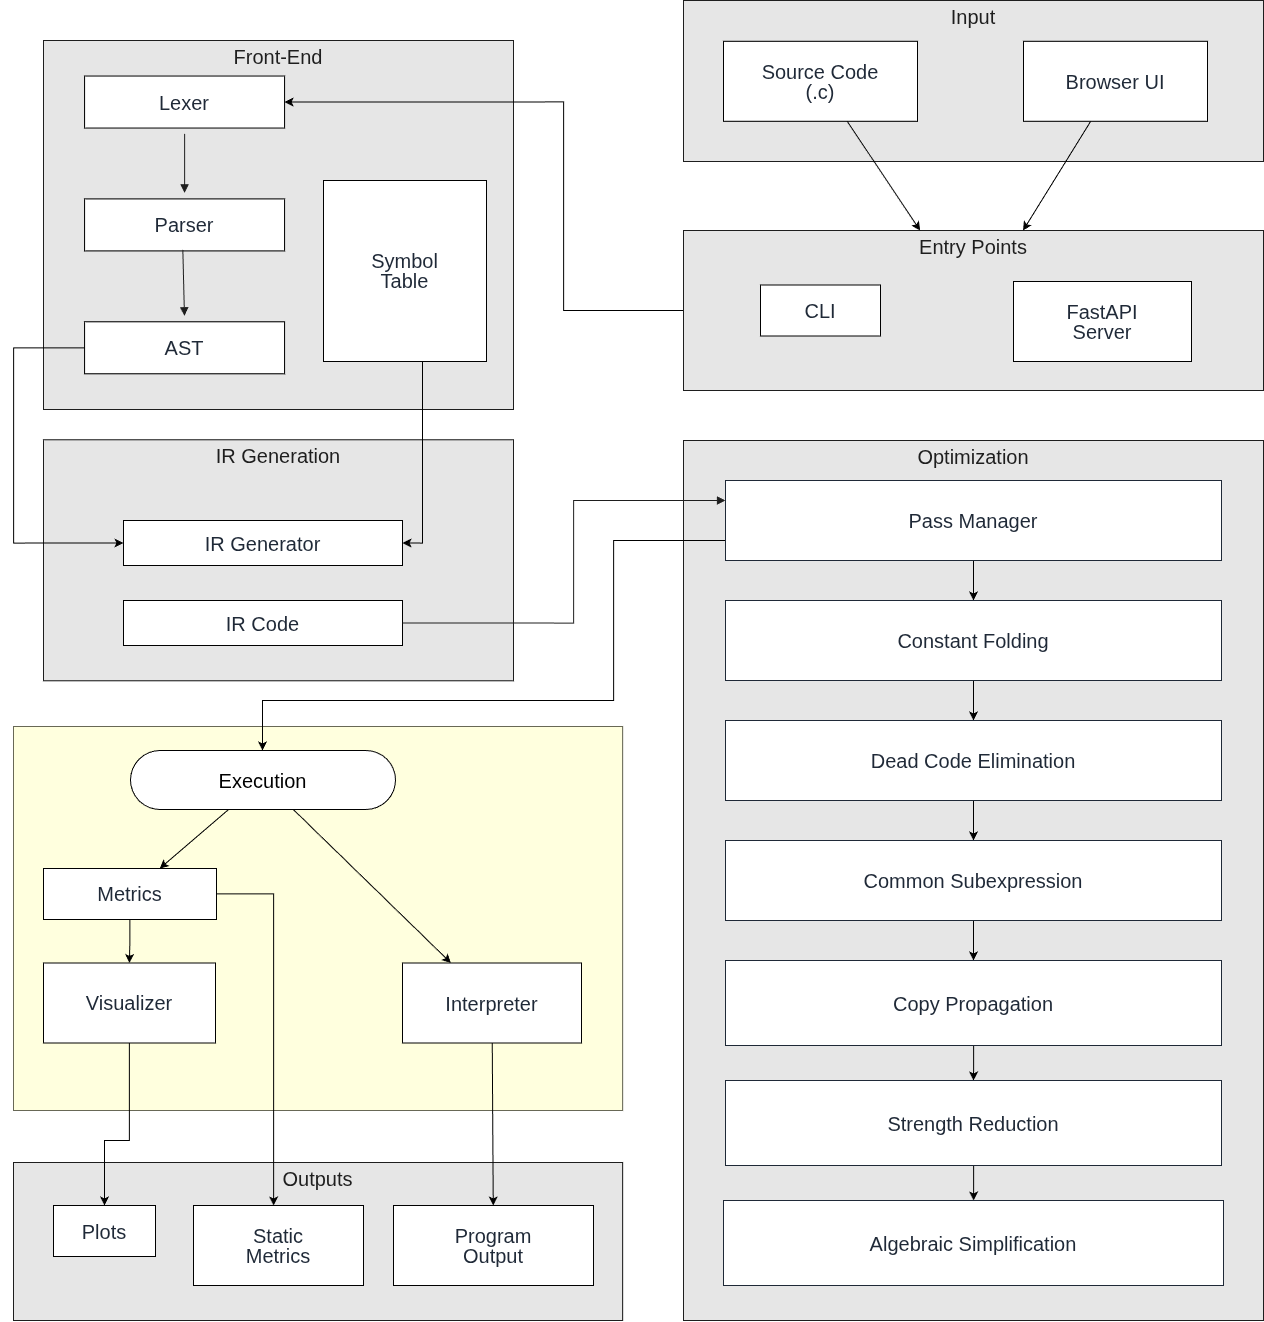
\includegraphics[width=\linewidth]{fig/arc.png}
    \caption{Component-Based Architecture of the Custom Compiler System showing the compilation pipeline and optimization framework.}
    \label{fig:architecture}
\end{figure}

\subsection{Intermediate Representation Design}
Three-Address Code was chosen as the IR because each instruction has at most one operator and two operands, which makes the local analyses the passes need (use and definition sets for DCE, an available-expression table for CSE) straightforward to implement and to read. The IR has 35 opcodes, of which seven (labels, no-ops, function begin and end markers, parameter declarations, and array and global declarations) are structural and produce no machine code.

\subsection{Configurable Pass Manager}
The Pass Manager accepts an ordered list of pass identifiers and applies them in sequence. Each pass receives the full IR and returns a new instruction list; the input is never mutated, so the same baseline IR is reused for all 720 orderings. The manager also records the IR and its size after each pass, which is how the per-pass figures in Section~\ref{sec:factorial} were obtained.

\subsection{Metrics and Cost Model}
\label{sec:metrics}
Three metrics are collected for every configuration.

\textit{Static code size} is the number of IR instructions excluding labels, no-ops, function markers, parameter declarations, and global declarations; an array declaration counts as one instruction but costs zero cycles.

\textit{Estimated execution cycles} is the sum, over the same instructions, of a per-opcode cost from Table~\ref{tab:cost_model}. The costs are approximate latencies for an ARM Cortex-M class in-order core, the kind of target MiBench represents: single-cycle ALU operations, a three-cycle multiplier, a twelve-cycle iterative divider, a two-cycle branch or load/store penalty, and fixed overheads for call, return, and the output routine. The model is static: it counts each instruction once regardless of how often it executes, and it does not model caches, pipelines, or branch prediction. It is used as a weighting of code size by instruction class rather than as a prediction of wall-clock time.

\textit{Dynamic instruction count} is the number of IR instructions actually executed by the interpreter on the program's fixed input. It is independent of the cost model and is the paper's model-free proxy for runtime.

\begin{table}[!htbp]
\centering
\caption{Per-instruction cost model used for the estimated-cycle metric}
\label{tab:cost_model}
\renewcommand{\arraystretch}{1.15}
{\small
\begin{tabularx}{\columnwidth}{@{}>{\raggedright\arraybackslash}Xc@{}}
\toprule
\textbf{IR opcodes} & \textbf{Cost} \\
\midrule
ADD, SUB, NEG, comparisons, AND, OR, NOT, COPY, LOAD\_CONST, PARAM & 1 \\
MUL & 3 \\
DIV, MOD & 12 \\
JUMP, JUMP\_IF\_TRUE, JUMP\_IF\_FALSE & 2 \\
ARR\_LOAD, ARR\_STORE, GLOBAL\_LOAD, GLOBAL\_STORE & 2 \\
CALL & 5 \\
RETURN & 3 \\
PRINT & 10 \\
LABEL, NOP, FUNC\_BEGIN, FUNC\_END, FUNC\_PARAM, ARR\_DECL, GLOBAL\_DECL & 0 \\
\bottomrule
\end{tabularx}
}
\end{table}

All percentages in this paper are reductions from the unoptimized baseline of the same program, $100 \times (1 - m_{\mathrm{opt}}/m_{\mathrm{base}})$, and all normalized values are the ratio $m_{\mathrm{opt}}/m_{\mathrm{base}}$, so that 1.0 is the baseline and smaller is better.

% --- SECTION VI: RESULTS AND DISCUSSION ---
\section{Results and Discussion}
Sections~\ref{sec:factorial} and~\ref{sec:interaction} follow one program, \texttt{factorial}, in detail, because its small size allows every number to be checked by hand. Sections~\ref{sec:classes} to~\ref{sec:validation} report the same measurements over all fifteen programs and all 720 orderings.

\subsection{Worked Example: the Factorial Benchmark}
\label{sec:factorial}
Listing~\ref{lst:factorial} shows the \texttt{factorial} source. It was written to contain all three kinds of opportunity: constant expressions (\texttt{base}, \texttt{extra}), dead assignments (\texttt{unused}, \texttt{also\_unused}), and a repeated subexpression (\texttt{base + extra}).

\begin{lstlisting}[basicstyle=\ttfamily\scriptsize,caption={The \texttt{factorial} benchmark (comments removed).},label={lst:factorial}]
int factorial(int n) {
    int result = 1;
    int i = 1;
    while (i <= n) {
        result = result * i;
        i = i + 1;
    }
    return result;
}
int main() {
    int base = 2 + 3;
    int extra = 10 - 5;
    int val = factorial(base);
    print(val);
    int unused = 42 * 2;
    int also_unused = unused + 100;
    int sum1 = base + extra;
    int sum2 = base + extra;
    print(sum1);
    print(sum2);
    return 0;
}
\end{lstlisting}

The IR generator places every literal in a temporary (\texttt{t6 = 2; t7 = 3; t8 = t6 + t7; base = t8}), which is why the unoptimized IR is larger than the source suggests. Its 40 countable instructions are 11 constant loads, 11 copies, 5 additions, 2 multiplications, 1 subtraction, 1 comparison, 2 jumps, 1 parameter push, 1 call, 2 returns, and 3 prints (13 in \texttt{factorial}, 27 in \texttt{main}). Under Table~\ref{tab:cost_model} these cost $30 \times 1 + 2 \times 3 + 2 \times 2 + 5 + 2 \times 3 + 3 \times 10 = 81$ estimated cycles. The best ordering leaves the loop in \texttt{factorial} at 10 instructions and reduces \texttt{main} to 6 (\texttt{param 5; t12 = call factorial; print t12; print 10; print 10; return 0}), for a total of 16 instructions and 55 estimated cycles.

Table~\ref{tab:phase_order_tradeoff} lists the baseline and six orderings. The 720 full orderings produce exactly six distinct outcomes on this program, and the six sequences were chosen so that each outcome appears once. AS is omitted from the listed sequences because it never changes the instruction count; appending it to any sequence leaves every entry in the table unchanged. Applying CF before DCE allows the removal of the constant-holding temporaries, whereas a DCE-first ordering removes only the seven planted dead instructions.

\begin{table}[!htbp]
\centering
\caption{Effect of Optimization Phase Ordering on Code Size and Estimated Cycles (Factorial Benchmark)}
\label{tab:phase_order_tradeoff}
\renewcommand{\arraystretch}{1.2}
{\footnotesize
\setlength{\tabcolsep}{4pt}
\begin{tabular}{@{}llcc@{}}
\toprule
\textbf{Label} & \textbf{Optimization Sequence} & \textbf{Size} & \textbf{Est. Cycles} \\
\midrule
Base  & Baseline (none) & 40 & 81 \\
Seq 1 & CF $\to$ CSE $\to$ CP $\to$ DCE $\to$ SR & 16 & 55 \\
Seq 2 & CSE $\to$ CP $\to$ CF $\to$ DCE $\to$ SR & 18 & 57 \\
Seq 3 & CP $\to$ CF $\to$ DCE $\to$ CSE $\to$ SR & 19 & 58 \\
Seq 4 & CF $\to$ DCE $\to$ CSE $\to$ CP $\to$ SR & 21 & 60 \\
Seq 5 & CP $\to$ DCE $\to$ CF $\to$ CSE $\to$ SR & 22 & 61 \\
Seq 6 & DCE $\to$ CF $\to$ CSE $\to$ CP $\to$ SR & 33 & 72 \\
\bottomrule
\end{tabular}
}
\end{table}

Fig.~\ref{fig:tradeoff_scatter} plots code size against estimated cycles for the six sequences. The best-performing sequence (Seq~1) occupies the lower-left corner, with a 60\% reduction in code size and a 32\% reduction in estimated cycles relative to the baseline. The per-pass log of the pass manager shows where the reduction happens: under Seq~1 the size stays at 40 through CF, CSE, and CP and drops to 16 at DCE. The enabling passes remove nothing themselves; they replace instructions by equivalents (a folded expression becomes a constant load, a recomputation becomes a copy, an operand is renamed) that leave other instructions unread, and DCE then deletes those. Run first, DCE finds only the planted dead code and the ordering ends at 33; run after CF but before CSE and CP (Seq~4), it ends at 21.

\begin{figure}[htbp]
    \centering
    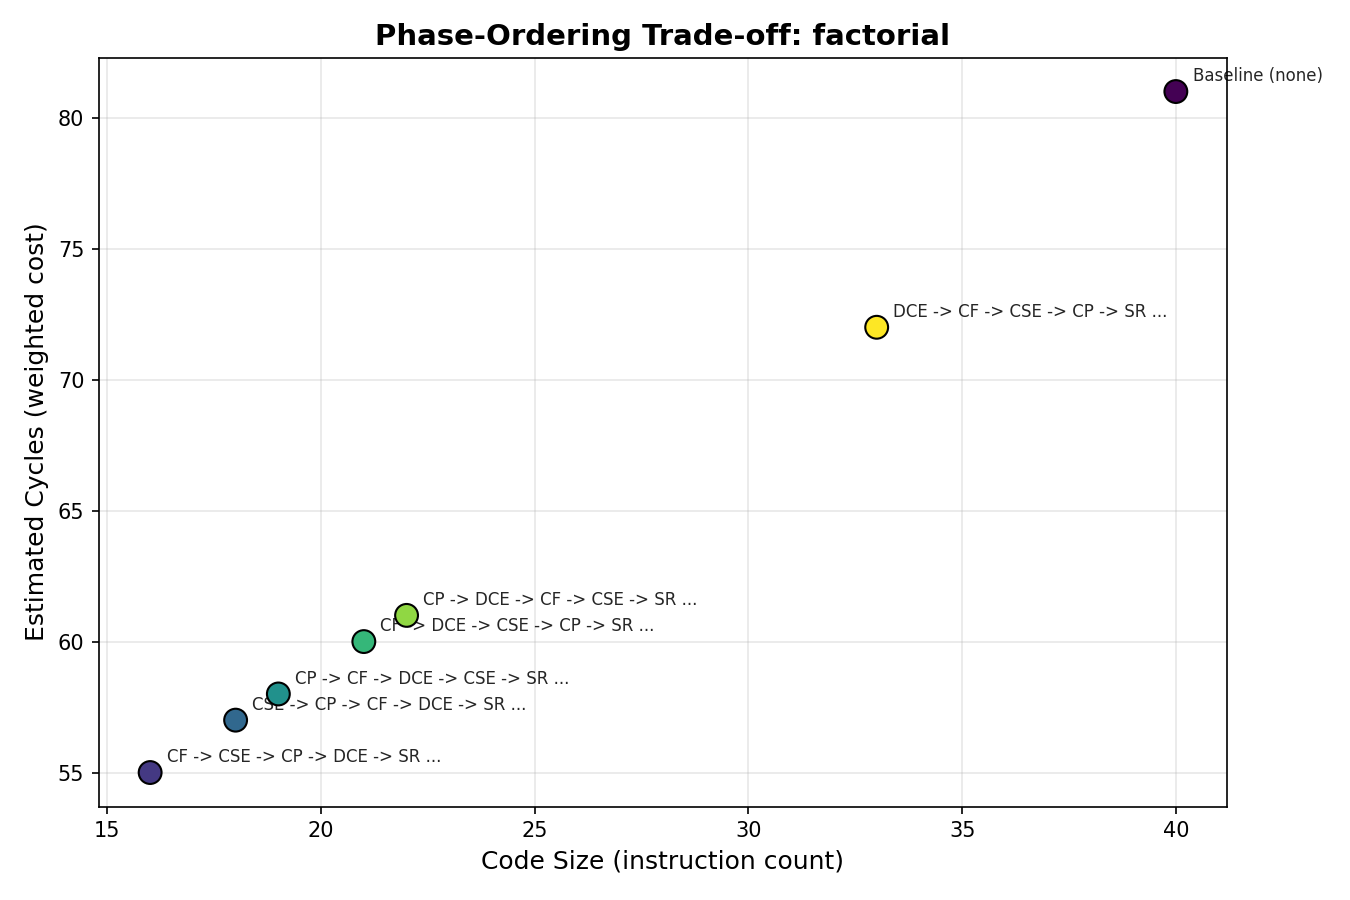
\includegraphics[width=0.8\columnwidth]{fig/factorial_tradeoff_scatter.png}
    \caption{Code size (instruction count) against estimated execution cycles for the six sequences of Table~\ref{tab:phase_order_tradeoff} and the baseline.}
    \label{fig:tradeoff_scatter}
\end{figure}

Table~\ref{tab:optimization_reduction} gives the three metrics for the six sequences as percentage reductions from the baseline (40 instructions, 81 estimated cycles, 81 executed instructions). Seq~1 (CF first) gives the largest reduction on all three metrics and Seq~6 (DCE first) the smallest.

\begin{table}[!htbp]
\centering
\caption{Optimization Effectiveness as Percentage Reduction from Baseline (Factorial Benchmark)}
\label{tab:optimization_reduction}
\renewcommand{\arraystretch}{1.2}
\begin{tabularx}{\columnwidth}{@{}Xccc@{}}
\toprule
\textbf{Sequence} & \textbf{Code Size (\%)} & \textbf{Est. Cycles (\%)} & \textbf{Dyn. Insts (\%)} \\
\midrule
Seq 1 & 60.0 & 32.1 & 34.6 \\
Seq 2 & 55.0 & 29.6 & 32.1 \\
Seq 3 & 52.5 & 28.4 & 30.9 \\
Seq 4 & 47.5 & 25.9 & 28.4 \\
Seq 5 & 45.0 & 24.7 & 27.2 \\
Seq 6 & 17.5 & 11.1 & 8.6 \\
\bottomrule
\end{tabularx}
\end{table}

\subsection{Pairwise Pass Interactions}
\label{sec:interaction}
Table~\ref{tab:pass_interaction} is computed from all 720 full orderings on \texttt{factorial}, not from the six sequences of Table~\ref{tab:phase_order_tradeoff}. For each ordered pair of passes $(A, B)$, the entry is the mean static code size, in IR instructions, over the 360 orderings in which $A$ runs before $B$ minus the mean over the 360 orderings in which $B$ runs before $A$. A negative entry means that running the row pass before the column pass gives smaller code; the matrix is antisymmetric by construction. Fig.~\ref{fig:pass_interaction} shows the same matrix rounded to integers.

\begin{table}[!htbp]
\centering
\caption{Pairwise interaction matrix for \texttt{factorial}: mean code size with row pass before column pass minus the reverse (IR instructions, over 720 orderings)}
\label{tab:pass_interaction}
\renewcommand{\arraystretch}{1.2}
{\small
\begin{tabularx}{\columnwidth}{@{}Xcccccc@{}}
\toprule
\textbf{A before B} & \textbf{AS} & \textbf{CF} & \textbf{CP} & \textbf{CSE} & \textbf{DCE} & \textbf{SR} \\
\midrule
AS  & 0      & $+$2.9 & $+$2.2 & $+$0.1 & $-$5.2  & 0 \\
CF  & $-$2.9 & 0      & $-$1.2 & $-$2.8 & $-$10.7 & $-$2.9 \\
CP  & $-$2.2 & $+$1.2 & 0      & $-$2.0 & $-$10.2 & $-$2.2 \\
CSE & $-$0.1 & $+$2.8 & $+$2.0 & 0      & $-$5.3  & $-$0.1 \\
DCE & $+$5.2 & $+$10.7 & $+$10.2 & $+$5.3 & 0     & $+$5.2 \\
SR  & 0      & $+$2.9 & $+$2.2 & $+$0.1 & $-$5.2  & 0 \\
\bottomrule
\end{tabularx}
}
\end{table}

The CF and CP rows against the DCE column carry the largest effects: placing CF before DCE saves 10.7 instructions on average out of 40, and CP before DCE saves 10.2. Two cautions apply to reading the matrix. First, it is a marginal statistic that averages over the positions of the other four passes, so an entry is not a causal effect of the pair alone; the AS and SR rows are non-zero even though neither pass ever changes the instruction count, because in the population of orderings ``AS before CF'' is correlated with ``DCE relatively later''. Second, the units are instructions of this one program. The equivalence-class analysis in Section~\ref{sec:classes}, which holds the other passes fixed, is the tool for attribution; the matrix is a quick view of which pairs matter most.

\begin{figure}[htbp]
    \centering
    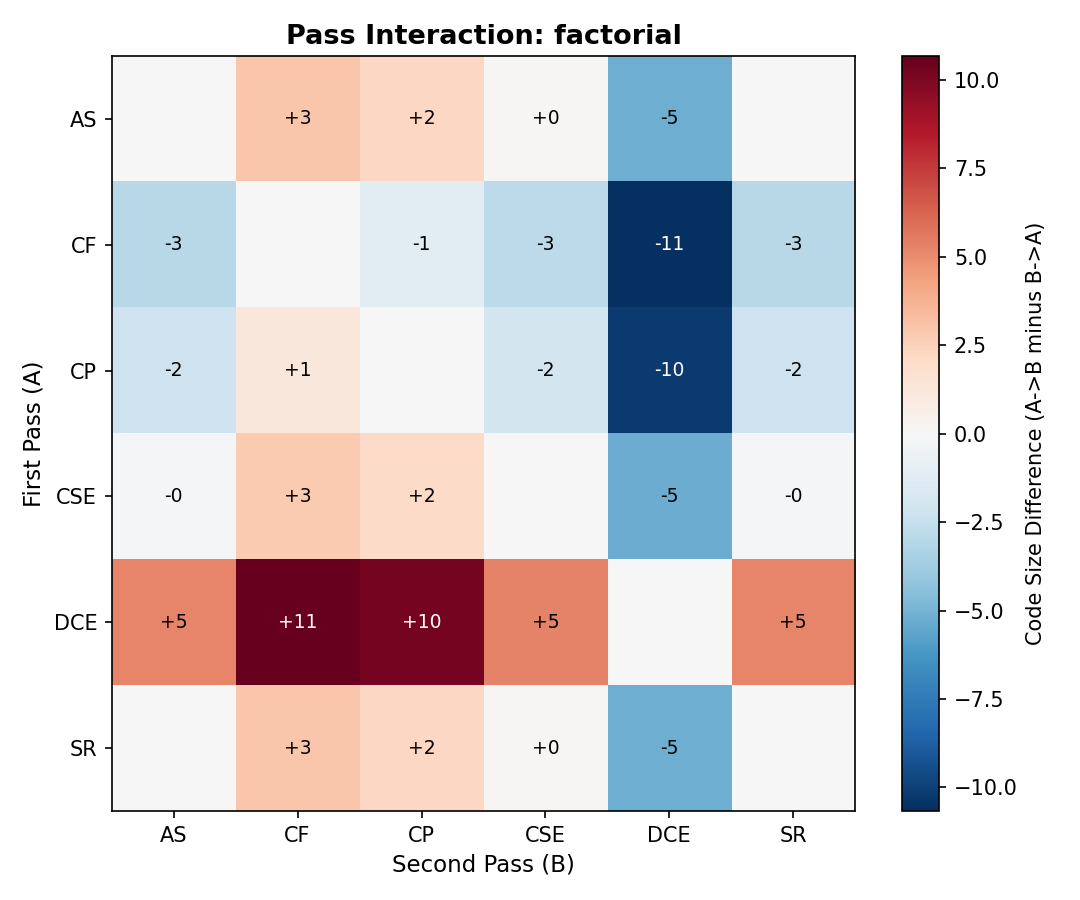
\includegraphics[width=0.8\columnwidth]{fig/factorial_pass_interaction.png}
    \caption{Heatmap of Table~\ref{tab:pass_interaction}: code size difference when applying pass A before pass B versus the reverse order, rounded to integers.}
    \label{fig:pass_interaction}
\end{figure}

\subsection{Generalization Across Fifteen Benchmarks}
\label{sec:classes}
Table~\ref{tab:per_program} reports, for each of the fifteen programs, the baseline and best static sizes and the reduction in all three metrics under the best ordering, together with the number of the 720 orderings that reach the best size. The best ordering has the same relative order of the four size-relevant passes, CF $\to$ CSE $\to$ CP $\to$ DCE, on every program, and it minimizes all three metrics simultaneously on every program. Across the suite it reduces code size by a geometric mean of 35.7\%, estimated cycles by 20.5\%, and executed instructions by 23.2\%.

\begin{table}[!htbp]
\centering
\caption{Baseline and best-ordering results for each program. Red.\ = percentage reduction under the best ordering; Opt.\ = number of the 720 orderings that reach the best code size.}
\label{tab:per_program}
\renewcommand{\arraystretch}{1.1}
{\footnotesize
\setlength{\tabcolsep}{3pt}
\begin{tabular}{@{}llrrrrrr@{}}
\toprule
 & & \multicolumn{2}{c}{\textbf{Size}} & \multicolumn{3}{c}{\textbf{Red.\ (\%)}} & \\
\cmidrule(lr){3-4}\cmidrule(lr){5-7}
\textbf{Program} & \textbf{Source} & base & best & Size & Cyc. & Dyn. & \textbf{Opt.} \\
\midrule
factorial & MiBench basicmath   & 40  & 16  & 60.0 & 32.1 & 34.6 & 120 \\
isqrt     & MiBench automotive  & 50  & 27  & 46.0 & 21.6 & 15.3 & 120 \\
bitcount  & MiBench automotive  & 33  & 19  & 42.4 & 15.9 & 33.6 & 360 \\
fibonacci & MiBench basicmath   & 22  & 13  & 40.9 & 25.7 & 19.9 & 240 \\
collatz   & MiBench automotive  & 42  & 26  & 38.1 & 14.2 & 32.2 & 360 \\
sha\_mix  & MiBench security    & 106 & 68  & 35.8 & 14.9 & 24.8 & 360 \\
jacobi1d  & PolyBench stencils  & 76  & 50  & 34.2 & 26.6 & 29.0 & 30 \\
jacobi2d  & PolyBench stencils  & 144 & 95  & 34.0 & 33.9 & 26.3 & 90 \\
power     & MiBench security    & 71  & 47  & 33.8 & 11.9 & 26.0 & 360 \\
gcd       & MiBench basicmath   & 21  & 14  & 33.3 & 13.7 & 22.2 & 360 \\
gemm      & PolyBench blas      & 164 & 119 & 27.4 & 21.3 & 15.9 & 30 \\
2mm       & PolyBench kernels   & 252 & 185 & 26.6 & 21.2 & 16.0 & 30 \\
gesummv   & PolyBench blas      & 106 & 78  & 26.4 & 20.0 & 18.8 & 30 \\
atax      & PolyBench kernels   & 101 & 78  & 22.8 & 14.6 & 12.9 & 30 \\
bicg      & PolyBench kernels   & 94  & 73  & 22.3 & 15.7 & 15.7 & 30 \\
\midrule
\multicolumn{4}{@{}l}{\textbf{Geometric mean reduction}} & \textbf{35.7} & \textbf{20.5} & \textbf{23.2} & \\
\bottomrule
\end{tabular}
}
\end{table}

Two groups are visible in Table~\ref{tab:per_program}. The scalar MiBench-derived programs are reduced by 33\% to 60\% in size, the array-based PolyBench-derived programs by 22\% to 34\%. In the scalar kernels a large share of the baseline is literal-holding temporaries and copies into named variables, which CF and CP make unread and DCE removes. In the array kernels the loop bodies are dominated by array loads and stores, which are never deleted without alias analysis, and by index arithmetic on variables reassigned every iteration, which are not constant-propagation candidates. The cycle reductions are smallest on the division-heavy programs \texttt{power} and \texttt{gcd}, because division costs twelve cycles in the model and its loop-carried operands keep it from ever being removed.

Fig.~\ref{fig:box} shows the distribution of code-size reduction over all 720 orderings for each program. The lower whisker reaches zero on thirteen of the fifteen programs: the worst orderings achieve nothing at all. Only the two programs with planted dead code have a non-zero floor.

\begin{figure*}[!t]
    \centering
    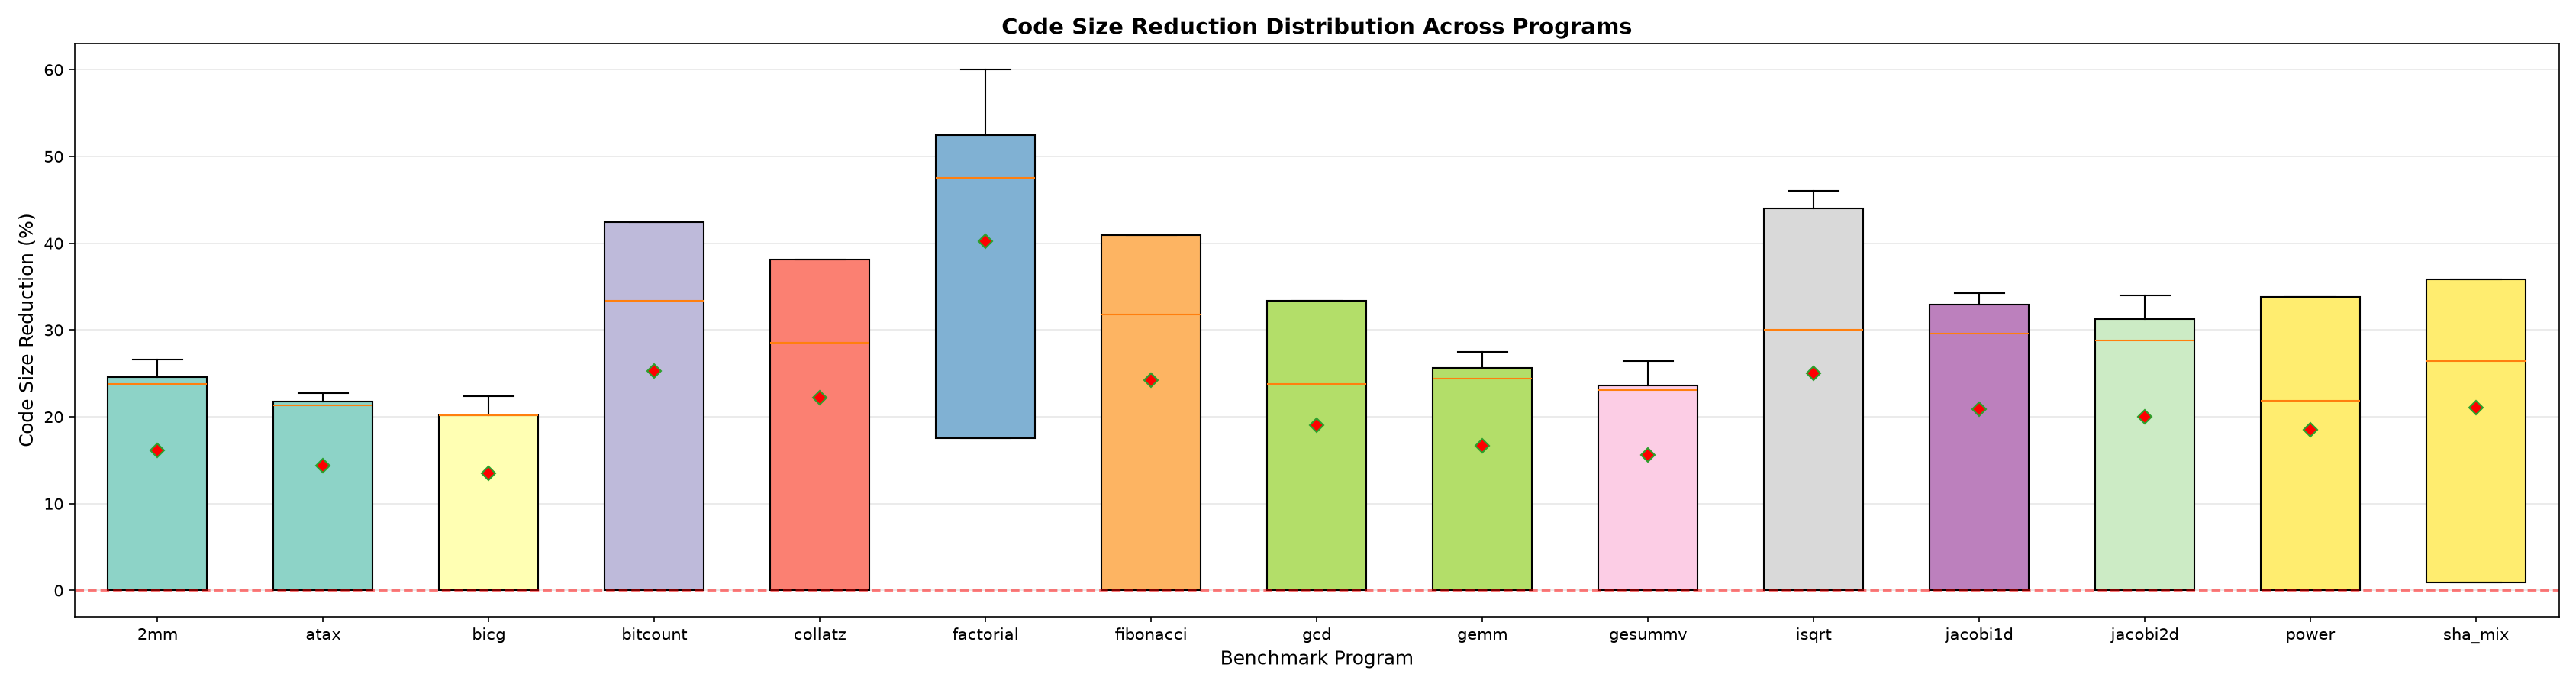
\includegraphics[width=0.92\textwidth]{fig/cross_program_box.png}
    \caption{Distribution of code-size reduction across all 720 orderings for each of the fifteen programs. Diamonds mark the mean. The lower whisker touches zero on every program except \texttt{factorial} and \texttt{sha\_mix}.}
    \label{fig:box}
\end{figure*}

\textbf{Equivalence classes.} Aggregated over the fifteen programs, the 720 orderings produce only nine distinct code-size outcomes (Table~\ref{tab:classes}). Each outcome is a class of orderings that produce identical code on every program, and the classes are determined entirely by the relative order of CF, CSE, CP, and DCE; the positions of SR and AS never change the instruction count. The $4! = 24$ relative orders each contain $720/24 = 30$ orderings and map onto nine classes, which is why the class sizes are multiples of 30. The cycle ratio varies within a class by less than 0.007, because SR rewrites $x \times 2$ as $x + x$ only when the literal is already in the instruction, which requires CF to have run first.

\begin{table}[!htbp]
\centering
\caption{The nine equivalence classes of orderings, by geometric-mean normalized code size over the fifteen programs (baseline = 1.0)}
\label{tab:classes}
\renewcommand{\arraystretch}{1.15}
{\footnotesize
\setlength{\tabcolsep}{2.5pt}
\begin{tabular}{@{}clrccc@{}}
\toprule
\textbf{Class} & \textbf{Relative order (number of orders)} & \textbf{$n$} & \textbf{Size} & \textbf{Cyc.} & \textbf{Dyn.} \\
\midrule
1 & CF $\to$ CSE $\to$ CP $\to$ DCE & 30 & 0.643 & 0.795 & 0.768 \\
2 & CSE $\to$ CF $\to$ CP $\to$ DCE & 30 & 0.646 & 0.798 & 0.773 \\
3 & CF $\to$ CP, then CSE/DCE either way (2) & 60 & 0.651 & 0.801 & 0.782 \\
4 & CSE $\to$ CP $\to$ CF $\to$ DCE & 30 & 0.653 & 0.801 & 0.775 \\
5 & CP first, CF before DCE (3) & 90 & 0.660 & 0.804 & 0.785 \\
6 & CSE $\to$ CP $\to$ DCE $\to$ CF & 30 & 0.684 & 0.818 & 0.787 \\
7 & CP first, DCE before CF (3) & 90 & 0.691 & 0.821 & 0.797 \\
8 & CF before DCE before CP (4) & 120 & 0.753 & 0.839 & 0.815 \\
9 & DCE before both CF and CP (8) & 240 & 0.987 & 0.962 & 0.994 \\
\bottomrule
\end{tabular}
}
\end{table}

The table reads as a set of rules that hold on every program. \textbf{DCE must follow CF and CP.} The eight relative orders in which DCE precedes both form class~9, a third of the whole space, with a size ratio of 0.987; on thirteen programs these 240 orderings leave the code unchanged, and the 1.3\% they achieve comes entirely from the planted dead code in two programs. DCE removes only instructions whose results are unread, and in the baseline IR every temporary is read at least once; CF and CP are what make temporaries unread. \textbf{DCE after CF but before CP (class~8) loses a third of the benefit}, because CP is what makes copies such as \texttt{sum1 = t18} unread. \textbf{CF before CP beats CP before CF} (class~1 against class~5), because CF substitutes through single-assignment variables to a fixed point whereas CP substitutes within a basic block only. \textbf{CSE between CF and CP is best} (class~1 against classes~2 to~4): CSE matches more expressions after CF has replaced temporaries by literals, and the copies CSE creates shrink the code only if CP then propagates them and DCE deletes them.

The marginal view agrees. Averaged over the fifteen programs and all orderings in which a pass runs first versus last, the mean size ratio moves from 0.988 (DCE first) to 0.659 (DCE last), from 0.873 (CP last) to 0.681 (CP first), and from 0.841 (CF last) to 0.707 (CF first); CSE's position barely matters (0.789 against 0.793), and SR and AS have no effect (0.791 in both positions).

\subsection{Statistical Significance}
\label{sec:stats}
The tests described in Section~\ref{sec:analysis} were applied to the per-program normalized metrics. The Friedman test over the 24 relative orders, with the fifteen programs as blocks, rejects the hypothesis that orderings are equivalent for all three metrics: code size $\chi^2(23) = 304.6$, $p = 5.3 \times 10^{-51}$, Kendall's $W = 0.88$; estimated cycles $\chi^2(23) = 296.0$, $p = 3.0 \times 10^{-49}$, $W = 0.86$; dynamic count $\chi^2(23) = 303.6$, $p = 8.5 \times 10^{-51}$, $W = 0.88$. A $W$ near 1 means that the fifteen programs rank the orderings almost identically, which is the statistical statement of the claim that the class structure is program-independent.

The post-hoc comparison of class~1 against class~9 (DCE first) is an exact Wilcoxon signed-rank test on fifteen paired size ratios: $W = 0$, $p = 3.1 \times 10^{-5}$ (one-sided), $r = 1.00$, median paired difference 0.34 of the baseline size. Class~1 is smaller on all fifteen programs, so the test statistic is at its minimum and the $p$-value is the smallest attainable with $n = 15$. Because these tests treat programs as the unit of replication, they say nothing about programs outside the suite; they establish that the ordering effect is not an artefact of one or two benchmarks.

\subsection{Trade-off Between Code Size and Execution Performance}
\label{sec:tradeoff}
Within this pass set there is no trade-off between the two objectives at the level of ordering classes. The class with the smallest code is also the class with the lowest estimated cycles and the lowest dynamic count on all fifteen programs (Tables~\ref{tab:per_program} and~\ref{tab:classes}). Over the 10,800 optimized runs, Spearman's $\rho$ between normalized size and normalized cycles is 0.79 and between size and dynamic count is 0.88; per program, the median $\rho$ between size and cycles is 1.00 and the minimum is 0.88. The residual trade-off is within a class and is caused by the position of SR relative to CF: in class~1, orderings with SR after CF have a geometric-mean cycle ratio of 0.7950 and orderings with SR before CF have 0.7999, a difference of 0.5\% with no change in size. The Pareto front of size against cycles is therefore short on every program, and a single ordering dominates every other class.

This finding is narrower than the conflict between size and time reported in LLVM-based studies \cite{ref8}. The six passes here are all code-shrinking transformations with no loop unrolling, inlining, or scheduling, which are the passes that trade size for speed; the result should be read as a property of this pass set, not of phase ordering in general.

\subsection{Validation and Limitations}
\label{sec:validation}
Every one of the 10,815 optimized programs printed the same output as its baseline and terminated. This is asserted by the benchmark driver and independently by the test suite. It is what allows the reductions above to be read as optimization rather than as accidental deletion: a soundness bug in any pass would appear as an output mismatch under some ordering, and one such bug in CSE was caught this way during development. As a further check, the baseline and class-1 IR of each program were lowered to RV32IM assembly and the assembly instructions counted: the reduction survives code generation with a geometric mean of 26.0\% (13.5\% on \texttt{bicg} to 50.4\% on \texttt{factorial}), smaller than the 35.7\% at the IR level because the back end has no register allocator and spends load and store instructions on every value.

Three limitations bound the claims. The cycle metric is a static cost model, not a hardware measurement; the dynamic instruction count is reported alongside it as a model-free second proxy, and the two agree in ranking ($\rho = 0.88$). The passes are block-local, so loop-carried copies such as \texttt{result = t3} survive in every loop of every benchmark; the measured reductions are a lower bound on what the same transformations would achieve with global data-flow analysis, and the class structure may change in that setting. The benchmarks are adapted kernels at fixed, small problem sizes; results for unmodified MiBench and PolyBench sources, or for pass sets that include loop and interprocedural transformations, are not established.

% --- SECTION VII: CONCLUSION ---
\section{Conclusion}
This paper studied the Phase Ordering Problem by exhaustive measurement on a small compiler built for the purpose, in which six classical passes are block-local, independently reorderable units under a configurable pass manager. All 720 orderings were applied to fifteen kernels adapted from MiBench and PolyBench/C, and every one of the 10,815 optimized programs was checked against its baseline output.

The order of passes matters by a large factor. The best family of orderings reduces static code size by a geometric mean of 35.7\%, estimated cycles by 20.5\%, and executed instructions by 23.2\%; the worst family, a third of all orderings, reduces code size by 1.3\% and leaves thirteen of the fifteen programs unchanged. The 720 orderings collapse into nine equivalence classes fixed by the relative order of four passes, and the effect is consistent across programs (Friedman $p < 10^{-48}$, Kendall's $W = 0.88$). The governing rule is that the passes which expose opportunities, Constant Folding and Copy Propagation, must run before the pass that consumes them, Dead Code Elimination, with Common Subexpression Elimination between them. On this pass set a single relative order is optimal for every program and for all three metrics at once; what varies by program is how many orderings reach the optimum, from 30 to 360 of 720, with the array kernels the least forgiving.

The framework is small enough to read in full and fast enough to re-run every experiment in under half a minute, and it can serve as a testbed for new passes, for search and learning methods evaluated against exhaustive ground truth, and for teaching.

% --- SECTION VIII: FUTURE WORK ---
\section{Future Work}
Possible extensions include:
\begin{itemize}
    \item Replace the static cost model with cycle counts measured on RISC-V hardware or a cycle-accurate simulator, using the existing RV32IM back end.
    \item Add global (CFG- or SSA-based) passes and loop transformations, and test whether the class structure survives.
    \item Evaluate unmodified MiBench and PolyBench sources at their standard problem sizes.
    \item Use the exhaustive results as ground truth for ML-guided phase ordering.
\end{itemize}

% --- REFERENCES ---
\begin{thebibliography}{33}

\bibitem{ref27}
A. H. Ashouri, S. S. G. Bagi, K. Satheeskumar, T. Srikanth, J. Zhao, I. Saidoun, Z. Wang, B. Chan, and T. S. Czajkowski,
``Protean compiler: An agile framework to drive fine-grain phase ordering,''
arXiv preprint, 2026.
\url{https://doi.org/10.48550/arXiv.2602.06142}

\bibitem{ref7}
J. Zhao \textit{et al.},
``Leveraging compilation statistics for compiler phase ordering,''
in \textit{Proceedings of the IEEE International Parallel and Distributed Processing Symposium (IPDPS)}, 2025.
\url{https://doi.org/10.1109/IPDPS64566.2025.00054}

\bibitem{ref25}
Y. Chen, H. Chen, Y. Yao, P. Yu, F. Xu, and X. Ma,
``Exploiting booster pass chain for compiler phase ordering,''
in \textit{Proc. 16th Int. Conf. Internetware}, 2025, pp. 175--185.
\url{https://doi.org/10.1145/3755881.3755899}

\bibitem{ref30}
R. Koitz-Hristov, F. Mandl, and F. Wotawa,
``VisOpt: Visualization of compiler optimizations for computer science education,''
in \textit{Proc. 56th ACM Technical Symp. Computer Science Education (SIGCSE TS)}, 2025, pp. 603--609.
\url{https://doi.org/10.1145/3641554.3701832}

\bibitem{ref1}
J. Liu \textit{et al.},
``Efficient compiler optimization by modeling passes dependence,''
\textit{CCF Transactions on High Performance Computing}, 2024.
\url{https://doi.org/10.1007/s42514-024-00197-9}

\bibitem{ref2}
R. Han and H. Kim,
``Exponentially expanding the phase-ordering search space via dormant information,''
in \textit{Proceedings of the ACM SIGPLAN Conference on Compiler Construction (CC)}, 2024.
\url{https://doi.org/10.1145/3640537.3641582}

\bibitem{ref3}
Y. Wang, H. Chen, and K. Wang,
``Beyond the phase ordering problem: Finding the globally optimal code with respect to optimization phases,''
arXiv preprint, 2024.
\url{https://doi.org/10.48550/arXiv.2410.03120}

\bibitem{ref4}
F. Huemer, D. Leopoldseder, A. Prokopec, R. Mosaner, and H. Mössenböck,
``Taking a closer look: An outlier-driven approach to compilation-time optimization,''
in \textit{Proceedings of the 38th European Conference on Object-Oriented Programming (ECOOP)}, 2024.
\url{https://doi.org/10.4230/LIPIcs.ECOOP.2024.20}

\bibitem{ref5}
H. Ahmed, M. F. Hyder, M. F. ul Haque, and P. C. Santos,
``Exploring compiler optimization space for control flow obfuscation,''
\textit{Computers \& Security}, 2024.
\url{https://doi.org/10.1016/j.cose.2024.103704}

\bibitem{ref6}
A. Schmitz \textit{et al.},
``Parallel pattern compiler for automatic global optimizations,''
\textit{Parallel Computing}, 2024.
\url{https://doi.org/10.1016/j.parco.2024.103112}

\bibitem{ref14}
F. Fernandes dos Santos, L. Carro, F. Vella, and P. Rech,
``Assessing the impact of compiler optimizations on GPUs reliability,''
\textit{ACM Transactions on Architecture and Code Optimization (TACO)},
vol. 21, no. 2, 2024.
\url{https://doi.org/10.1145/3638249}

\bibitem{ref13}
M. Tao,
``Semantic ontology enabled modeling, retrieval and inference for incomplete mobile trajectory data,''
\textit{Future Generation Computer Systems}, vol. 145, pp. 1--11, 2023.
\url{https://doi.org/10.1016/j.future.2023.03.012}

\bibitem{ref22}
M. Zhu and D. Hao,
``Compiler auto-tuning via critical flag selection,''
in \textit{Proceedings of the IEEE/ACM International Conference on Automated Software Engineering (ASE)}, 2023.
\url{https://doi.org/10.1109/ASE56229.2023.00209}

\bibitem{ref24}
A. Pe\v{c}im\'{u}th, D. Leopoldseder, and P. T\u{u}ma,
``Diagnosing compiler performance by comparing optimization decisions,''
in \textit{Proc. 20th ACM SIGPLAN Int. Conf. Managed Programming Languages and Runtimes (MPLR)}, 2023, pp. 47--61.
\url{https://doi.org/10.1145/3617651.3622994}

\bibitem{ref26}
R. Han and H. Kim,
``Exponentially expanding the compiler phase-ordering problem's search space through the learning of dormant information,''
2023.
\url{https://openreview.net/pdf?id=frjDLUebFY}

\bibitem{ref29}
C. Shewale, S. B. Shinde, Y. B. Gurav, R. J. Patil, and S. U. Kadam,
``Compiler optimization prediction with new self-improved optimization model,''
\textit{International Journal of Advanced Computer Science and Applications (IJACSA)}, vol. 14, no. 2, 2023.
\url{https://doi.org/10.14569/IJACSA.2023.0140267}

\bibitem{ref8}
S. Jain \textit{et al.},
``POSET-RL: Phase ordering for optimizing size and execution time using reinforcement learning,''
in \textit{Proceedings of the IEEE ISPASS}, 2022.
\url{https://doi.org/10.1109/ISPASS55109.2022.00012}

\bibitem{ref10}
M. Camilli, A. Janes, and B. Russo,
``Automated test-based learning and verification of performance models for microservices systems,''
\textit{Journal of Systems and Software}, vol. 187, 2022.
\url{https://doi.org/10.1016/j.jss.2022.111225}

\bibitem{ref11}
S. Zhang, X.-W. Guo, C. Li, Y. Liu, S. Fan, R. Zhao, and C. Yang,
``A large scale parallel fluid-structure interaction computing platform for simulating structural responses to a detonation shock,''
\textit{Software: Practice and Experience}, vol. 53, no. 1, pp. 211--240, 2023.
\url{https://doi.org/10.1002/spe.3051}

\bibitem{ref28}
H. Liu, J. Xu, S. Chen, and T. Guo,
``Compiler optimization parameter selection method based on ensemble learning,''
\textit{Electronics}, vol. 11, no. 15, 2022.
\url{https://doi.org/10.3390/electronics11152452}

\bibitem{ref23}
S. Kloibhofer,
``Run-time data analysis to drive compiler optimizations,''
in \textit{Companion Proc. ACM SIGPLAN SPLASH}, 2021, pp. 9--12.
\url{https://doi.org/10.1145/3484271.3484974}

\bibitem{ref9}
S. VenkataKeerthy \textit{et al.},
``IR2Vec: LLVM IR based scalable program embeddings,''
\textit{ACM Transactions on Architecture and Code Optimization (TACO)}, 2020.
\url{https://doi.org/10.1145/3418463}

\bibitem{ref12}
Q. Huang \textit{et al.},
``AutoPhase: Compiler phase-ordering for high-level synthesis,''
arXiv preprint, 2020.
\url{https://doi.org/10.48550/arXiv.2003.00671}

\bibitem{ref15}
A. H. Ashouri, A. Bignoli, G. Palermo, C. Silvano, S. Kulkarni, and J. Cavazos,
``MiCOMP: Mitigating the compiler phase-ordering problem using optimization subsequences and machine learning,''
\textit{ACM Transactions on Architecture and Code Optimization (TACO)}, vol. 14, no. 3, pp. 1--28, 2017.
\url{https://doi.org/10.1145/3124452}

\bibitem{ref17}
A. H. Ashouri, A. Bignoli, G. Palermo, and C. Silvano,
``Predictive modeling methodology for compiler phase-ordering,''
in \textit{Proc. PARMA-DITAM Workshops}, 2016, pp. 7--12.
\url{https://doi.org/10.1145/2872421.2872424}

\bibitem{ref20}
R. Nobre, L. G. A. Martins, and J. M. P. Cardoso,
``A graph-based iterative compiler pass selection and phase ordering approach,''
in \textit{Proc. 17th ACM SIGPLAN/SIGBED Conf. Languages, Compilers, Tools, and Theory for Embedded Systems (LCTES)}, 2016, pp. 21--30.
\url{https://doi.org/10.1145/2907950.2907959}

\bibitem{ref31}
L.-N. Pouchet,
``PolyBench/C: The polyhedral benchmark suite,'' version 4.2, 2016.
\url{https://web.cse.ohio-state.edu/~pouchet.2/software/polybench/}

\bibitem{ref16}
C. Lattner and V. Adve,
``LLVM: A compilation framework for lifelong program analysis and transformation,''
in \textit{Proceedings of the International Symposium on Code Generation and Optimization (CGO)}, 2004.
\url{https://doi.org/10.1109/CGO.2004.1281665}

\bibitem{ref19}
P. Kulkarni \textit{et al.},
``Fast searches for effective optimization phase sequences,''
\textit{ACM SIGPLAN Notices}, vol. 39, no. 6, pp. 171--182, 2004.
\url{https://doi.org/10.1145/996893.996863}

\bibitem{ref18}
K. D. Cooper, T. J. Harvey, and L. Torczon,
``Compiler-based code-improvement techniques,''
in \textit{Handbook of Computer Science and Engineering}, 2002.
\url{https://www.cs.tufts.edu/~nr/cs257/archive/keith-cooper/survey.pdf}

\bibitem{ref32}
M. R. Guthaus, J. S. Ringenberg, D. Ernst, T. M. Austin, T. Mudge, and R. B. Brown,
``MiBench: A free, commercially representative embedded benchmark suite,''
in \textit{Proceedings of the IEEE International Workshop on Workload Characterization (WWC-4)}, 2001.
\url{https://doi.org/10.1109/WWC.2001.990739}

\bibitem{ref21}
D. F. Bacon, S. L. Graham, and O. J. Sharp,
``Compiler transformations for high-performance computing,'' \textit{ACM Computing Surveys}, vol. 26, no. 4, pp. 345--420, 1994.
\url{https://doi.org/10.1145/197405.197406}

\bibitem{ref33}
P. J. Fleming and J. J. Wallace,
``How not to lie with statistics: The correct way to summarize benchmark results,''
\textit{Communications of the ACM}, vol. 29, no. 3, pp. 218--221, 1986.
\url{https://doi.org/10.1145/5666.5673}

\end{thebibliography}

\end{document}
